\chapter{Espectroscopia de rotación y de vibración}\label{ch:b3:rovibrational-spectroscopy}

En una meseta alta y seca, decenas de antenas de radio apuntan hacia una nube oscura
entre las estrellas. Entre las frecuencias que recogen hay una a
\qty{115.271}{GHz}: moléculas de monóxido de carbono, a unos pocos kelvin, que pasan
de su primer nivel de rotación al más bajo. De ese único número, un
químico obtiene la longitud del enlace C--O con una precisión de una fracción de picómetro; de
las intensidades de las rayas siguientes, la temperatura de la nube. Las
rotaciones y vibraciones de las moléculas son el objeto de este capítulo: sus
niveles, a partir del rotor y del oscilador del
\cref{ch:b3:quantum-model-systems}; las reglas de selección, a partir del
\cref{ch:b3:group-theory-applied}; y lo que miden los espectros: longitudes de
enlace, \omterm{def:b3:quantum-model-systems:oscillator}{constantes de fuerza}, energías de disociación.

\begin{recall}
El \cref{ch:b3:quantum-model-systems} dio el \omterm{def:b3:quantum-model-systems:rotor}{rotor rígido}, $E_J = J(J+1)\hbar^2/2I$,
con \omterm{def:b3:quantum-model-systems:degenerate}{degeneración} $2J + 1$, y el \omterm{def:b3:quantum-model-systems:oscillator}{oscilador armónico}, $E_v = (v + \frac12)h\nu$,
para una diatómica de \omterm{def:b3:quantum-model-systems:oscillator}{masa reducida} $\mu$. El \cref{ch:b3:group-theory-applied} enunció
las reglas de selección infrarroja y Raman. El volumen del primer año midió espectros
infrarrojos en números de onda y definió la polarizabilidad de una molécula.
\end{recall}

\begin{omfigure}
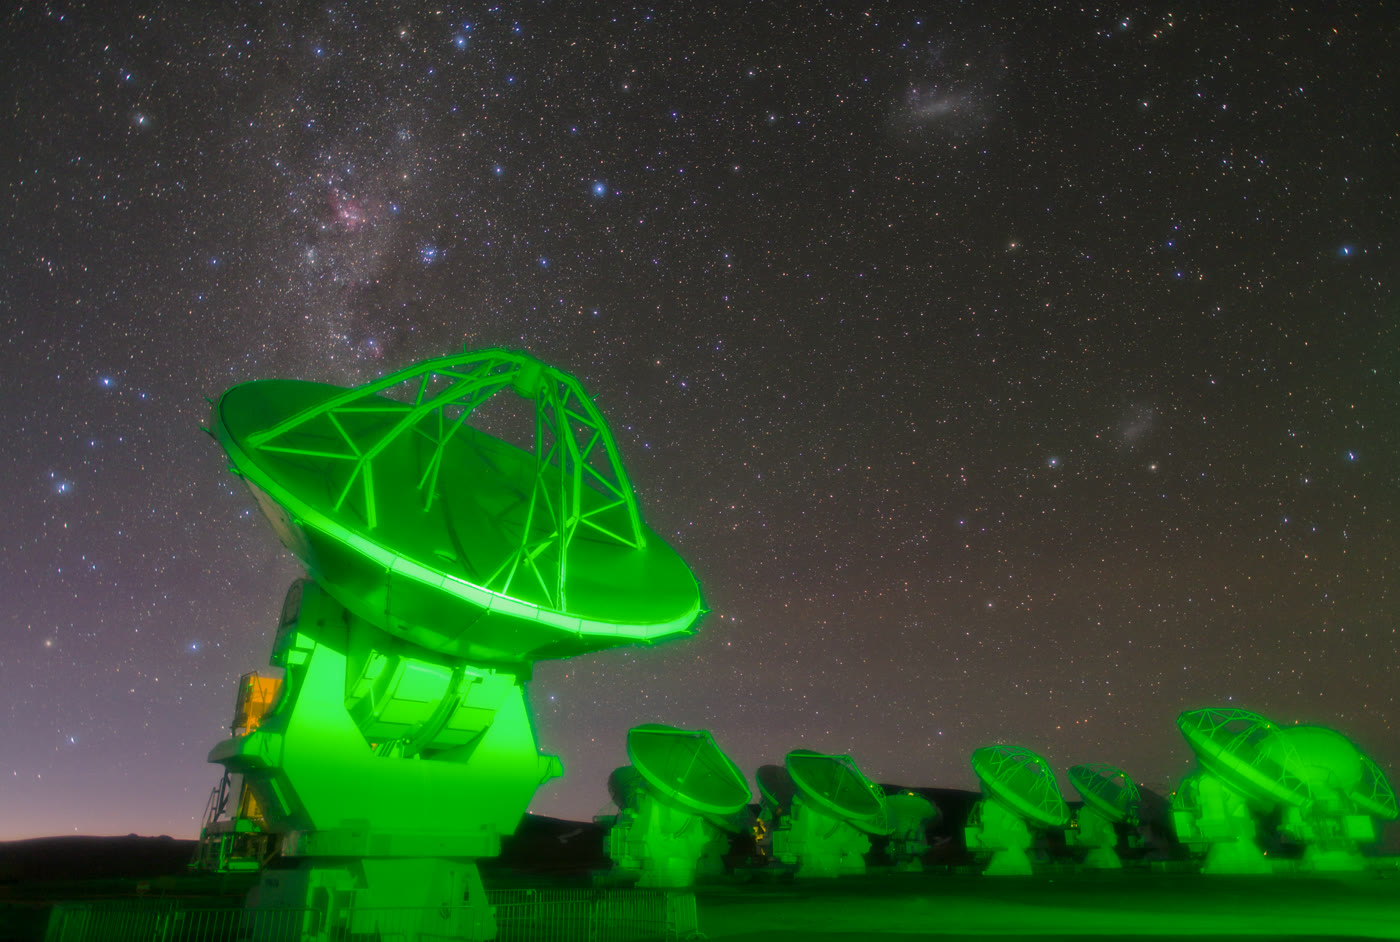
\includegraphics[width=0.7\linewidth]{images/book4/alma-antennas.jpg}

{\small Antenas de un radiointerferómetro en una meseta alta: registran,
entre muchas otras, las rayas de rotación del monóxido de carbono de las nubes
interestelares. Fotografía ESO/B.~Tafreshi (twanight.org), CC BY 4.0.}
\end{omfigure}

\section{Espectros de rotación}

\begin{definition}[Constante de rotación, isotopólogo]\label{def:b3:rovibrational-spectroscopy:rotational-constant}
La \emph{constante de rotación}\index{constante de rotacion@constante de rotación} de una molécula lineal
es $B = h/(8\pi^2cI)$, en \unit{cm^{-1}} (o $B = h/8\pi^2I$ en hercios), de modo que sus
niveles de rotación son $F(J) = BJ(J+1)$ en números de onda. Las moléculas que solo difieren
en los isótopos de sus átomos son \emph{isotopólogos}\index{isotopologo@isotopólogo}
(\ce{^{12}C^{16}O}, \ce{^{13}C^{16}O}); en la \omterm{def:b3:computational-chemistry:born-oppenheimer}{aproximación de Born--Oppenheimer}
comparten las mismas longitudes de enlace y las mismas \omterm{def:b3:quantum-model-systems:oscillator}{constantes de fuerza}.
\end{definition}

\begin{definition}[Reglas de selección general y específica]\label{def:b3:rovibrational-spectroscopy:selection}
Una \emph{regla de selección general}\index{regla de seleccion general@regla de selección general} indica qué
propiedad debe tener una molécula para presentar un tipo de espectro; una
\emph{regla de selección específica}\index{regla de seleccion especifica@regla de selección específica} indica qué
cambios de número cuántico están permitidos.
\end{definition}

\begin{proposition}[Espectros de rotación pura]\label{prop:b3:rovibrational-spectroscopy:rotational-lines}
Una molécula solo tiene un espectro de rotación pura (de microondas) si tiene un
momento dipolar permanente; para una molécula lineal, la regla específica es $\Delta J
= \pm1$. Las rayas de absorción están en
\[
\tilde\nu = F(J+1) - F(J) = 2B(J + 1), \qquad J = 0, 1, 2, \dots,
\]
equidistantes en $2B$.
\end{proposition}

\begin{proof}
La interacción con la luz se produce a través del momento dipolar: una molécula sin
dipolo permanente no tiene dipolo oscilante cuando gira. La regla $\Delta J
= \pm1$ procede de la anulación de $\int Y_{J'M'}^*\cos\theta\,Y_{JM}$ salvo si $J' = J
\pm 1$ (la componente del dipolo según $z$ se transforma como $Y_{1,0}$), que se admite.
Entonces $B(J+1)(J+2) - BJ(J+1) = 2B(J+1)$.
\end{proof}

\begin{method}[Longitud de enlace a partir de una raya de rotación]\label{met:b3:rovibrational-spectroscopy:bond-length}
\begin{enumerate}
  \item A partir de la raya $J + 1 \leftarrow J$ de frecuencia $\nu$, deducir $B =
        \nu/2(J+1)$ (en hercios).
  \item Calcular el momento de inercia $I = h/8\pi^2B$.
  \item Con la \omterm{def:b3:quantum-model-systems:oscillator}{masa reducida} obtenida de las masas isotópicas, $r = \sqrt{I/\mu}$.
\end{enumerate}
\end{method}

\begin{example}[El monóxido de carbono]\label{ex:b3:rovibrational-spectroscopy:co}
% ledger: rotl:CO.1-0, imass:O16
La raya $J = 1 \leftarrow 0$ de \ce{^{12}C^{16}O} está a \qty{115271.20}{MHz}:
$B = \qty{57635.6}{MHz} = \qty{1.92252}{cm^{-1}}$, $I = \qty{1.4560e-46}{kg.m^2}$.
Con $\mu = 12 \times 15.99491/27.99491 = \qty{6.85621}{u}$, $r_0 = \qty{113.09}{pm}$.
Este $r_0$ promedia el enlace sobre su vibración de punto cero y es algo más
largo que la longitud de equilibrio $r_e$ (\cref{sec:b3:rovibrational-spectroscopy:real-bonds}).
\end{example}

\begin{definition}[Constante de distorsión centrífuga]\label{def:b3:rovibrational-spectroscopy:centrifugal}
Un enlace que gira se alarga; los niveles pasan a ser $F(J) = BJ(J+1) - DJ^2(J+1)^2$,
donde $D$ es la \emph{constante de distorsión centrífuga}\index{constante de distorsion centrifuga@constante de distorsión centrífuga},
y las rayas $2B(J+1) - 4D(J+1)^3$ se van acercando lentamente a
$J$ alto.
\end{definition}

\begin{proposition}[La raya más intensa]\label{prop:b3:rovibrational-spectroscopy:jmax}
Si las intensidades de las rayas siguen la población del nivel inferior, $(2J+1)
\eu^{-hcBJ(J+1)/kT}$, el nivel más poblado está cerca de
\[
J_{\max} \approx \sqrt{\frac{kT}{2hcB}} - \frac12.
\]
\end{proposition}

\begin{proof}
Se trata $J$ como continuo y se deriva: $\frac{\dd}{\dd J}[(2J+1)\eu^{-aJ(J+1)}]
= [2 - a(2J+1)^2]\eu^{-aJ(J+1)}$ con $a = hcB/kT$; se anula en $(2J + 1)^2 =
2/a$.
\end{proof}

\begin{omfigure}
\begin{tikzpicture}
\begin{axis}[width=0.9\linewidth, height=4.8cm, xmin=0, xmax=70, ymin=0,
  ymax=1.12, ytick=\empty, axis x line=bottom, axis y line=left, ycomb,
  xlabel={número de onda / cm$^{-1}$}, ylabel={intensidad relativa},
  tick label style={font=\small}, label style={font=\small}]
\addplot[omDef, very thick] table[x=nu, y=I] {figdata/out/bachelor-3-rotational-spectrum-co-30.dat};
\addplot[omThm, thick, xshift=1.2pt] table[x=nu, y=I] {figdata/out/bachelor-3-rotational-spectrum-co-300.dat};
\end{axis}
\end{tikzpicture}

{\small El espectro de absorción de rotación del monóxido de carbono, con rayas separadas
$2B = \qty{3.845}{cm^{-1}}$ e intensidades tomadas iguales a la población del
nivel inferior, a \qty{30}{K} (azul) y a \qty{300}{K} (rojo, ligeramente desplazado para
que se vea), con cada temperatura escalada a su raya más intensa. A \qty{30}{K}, la raya más intensa es
$J = 3 \leftarrow 2$; a \qty{300}{K}, $J = 8 \leftarrow 7$.}
\end{omfigure}

\section{Vibraciones de enlaces reales}\label{sec:b3:rovibrational-spectroscopy:real-bonds}

Un enlace real no obedece a la ley de Hooke lejos del equilibrio: se ablanda al
estirarse y se rompe.

\begin{definition}[Potencial de Morse]\label{def:b3:rovibrational-spectroscopy:morse}
El \emph{potencial de Morse}\index{potencial de Morse} es $V(r) = D_e[1 -
\eu^{-\beta(r - r_e)}]^2$: armónico cerca de $r_e$ (\omterm{def:b3:quantum-model-systems:oscillator}{constante de fuerza} $2\beta^2D_e$), y
tiende al límite de disociación $D_e$ para $r$ grande.
\end{definition}

\begin{proposition}[Niveles del oscilador de Morse]\label{prop:b3:rovibrational-spectroscopy:morse-levels}
En números de onda, los niveles de vibración de un oscilador de Morse son
\[
G(v) = \tilde\omega_e(v + \tfrac12) - \tilde\omega_ex_e(v + \tfrac12)^2, \qquad
\tilde\omega_ex_e = \frac{\tilde\omega_e^2}{4D_e},
\]
una escalera cuyos peldaños se acercan y terminan en $v_{\max} = \lfloor\tilde\omega_e/
2\tilde\omega_ex_e - \frac12\rfloor$.
\end{proposition}
\admitted

La resolución de la ecuación de Morse corresponde a cursos más avanzados;
los niveles se comprueban numéricamente en los datos de las figuras de este capítulo.

\begin{definition}[Constante de anarmonicidad, fundamental, sobretono, banda caliente]\label{def:b3:rovibrational-spectroscopy:anharmonic}
$\tilde\omega_ex_e$ es la \emph{constante de anarmonicidad}\index{constante de anarmonicidad}.
La \emph{transición fundamental}\index{transicion fundamental@transición fundamental}
es $v = 1 \leftarrow 0$; un \emph{sobretono}\index{sobretono} es $v = n \leftarrow 0$
con $n \ge 2$, débil porque la regla general $\Delta v = \pm1$ del \omterm{def:b3:quantum-model-systems:oscillator}{oscilador
armónico} solo se incumple ligeramente; una \emph{banda caliente}\index{banda caliente} parte
de un nivel excitado, $v = 2 \leftarrow 1$, y crece con la temperatura.
\end{definition}

\begin{definition}[Energía de disociación espectroscópica]\label{def:b3:rovibrational-spectroscopy:dissociation}
La \emph{energía de disociación espectroscópica}\index{energia de disociacion espectroscopica@energía de disociación espectroscópica}
de una molécula es la profundidad de su potencial, $D_e$, medida desde el
mínimo, o $D_0 = D_e - G(0)$, medida desde el nivel más bajo ---por
molécula y a \qty{0}{K}, a diferencia de la entalpía de disociación de enlace del volumen del segundo
año, una entalpía molar a \qty{298}{K}.
\end{definition}

\begin{corollary}[$D_e$ y $D_0$ de un oscilador de Morse]\label{cor:b3:rovibrational-spectroscopy:de}
$D_e = \tilde\omega_e^2/4\tilde\omega_ex_e$ y $D_0 = D_e - (\frac12\tilde\omega_e -
\frac14\tilde\omega_ex_e)$.
\end{corollary}

\begin{proof}
La primera es la relación de la proposición; la segunda es $G(0)$.
\end{proof}

\begin{proposition}[Extrapolación de Birge--Sponer]\label{prop:b3:rovibrational-spectroscopy:birge-sponer}
Las separaciones $\Delta G(v + \frac12) = G(v+1) - G(v) = \tilde\omega_e - 2\tilde\omega_ex_e(v +
1)$ disminuyen linealmente con $v$; sumarlas hasta que se anulan da $D_0$, el
área bajo la gráfica de $\Delta G$ en función de $v$.
\end{proposition}

\begin{proof}
Se restan las dos expresiones de $G$. $D_0$ es la energía desde $v = 0$ hasta el
límite, la suma de todas las separaciones.
\end{proof}

\begin{example}[El cloruro de hidrógeno]\label{ex:b3:rovibrational-spectroscopy:hcl}
% ledger: diat:HCl.we, diat:HCl.wexe, janaf:H.dfH0, janaf:Cl.dfH0, janaf:HCl.dfH0
Para \ce{H^{35}Cl}, $\tilde\omega_e = \qty{2990.95}{cm^{-1}}$ y $\tilde\omega_ex_e =
\qty{52.82}{cm^{-1}}$: la fundamental está en $\tilde\omega_e - 2\tilde\omega_ex_e =
\qty{2885.3}{cm^{-1}}$ y el primer \omterm{def:b3:rovibrational-spectroscopy:anharmonic}{sobretono} en $2\tilde\omega_e - 6\tilde\omega_ex_e =
\qty{5665.0}{cm^{-1}}$, algo menos del doble de la fundamental. El modelo de Morse
predice $D_e = \qty{42342}{cm^{-1}}$ y $D_0 = \qty{40860}{cm^{-1}}$; el $D_0$ verdadero,
obtenido de las entalpías de formación de H, Cl y HCl a \qty{0}{K}, es
\qty{35760}{cm^{-1}} (\qty{4.43}{eV}). El potencial real se aplana más deprisa que una
curva de Morse ajustada en el fondo: las extrapolaciones de Birge--Sponer a partir de los
niveles más bajos sobrestiman las energías de disociación.
\end{example}

\begin{omfigure}
\begin{tikzpicture}
\begin{axis}[name=morse, width=0.55\linewidth, height=6cm, xmin=0.8, xmax=4.0,
  ymin=0, ymax=48000, axis lines=left, xlabel={$r$ / \AA}, ylabel={$V$ / cm$^{-1}$},
  unbounded coords=jump, scaled y ticks=false, ytick={0,10000,20000,30000,40000},
  tick label style={font=\small}, label style={font=\small}]
\addplot[black, thick] table[x=r, y=V] {figdata/out/bachelor-3-morse-levels.dat};
\addplot[gray, dashed] table[x=r, y=harm] {figdata/out/bachelor-3-morse-levels.dat};
\addplot[omDef] table[x=r, y=E] {figdata/out/bachelor-3-morse-levels-levels.dat};
\draw[<->, omThm] (axis cs:3.7,0) -- (axis cs:3.7,42342) node[pos=0.5, left, font=\small] {$D_e$};
\draw[dashed, omThm] (axis cs:1.2,42342) -- (axis cs:4.0,42342);
\end{axis}
\begin{axis}[at={(morse.east)}, anchor=west, xshift=1.6cm, width=0.4\linewidth,
  height=5cm, xmin=0, xmax=28, ymin=0, ymax=3100, axis lines=left,
  xlabel={$v$}, ylabel={$\Delta G(v + \frac12)$ / cm$^{-1}$},
  tick label style={font=\small}, label style={font=\small}]
\addplot[omDef, only marks, mark size=1.2pt] table[x=v, y=dG] {figdata/out/bachelor-3-morse-levels-bs.dat};
\addplot[omDef!40, fill=omDef!12, draw=none] table[x=v, y=dG] {figdata/out/bachelor-3-morse-levels-bs.dat} \closedcycle;
\end{axis}
\end{tikzpicture}

{\small Izquierda: el \omterm{def:b3:rovibrational-spectroscopy:morse}{potencial de Morse} de \ce{HCl} construido a partir de sus constantes
espectroscópicas (trazo continuo), la parábola armónica de la misma curvatura (trazo discontinuo)
y uno de cada tres niveles de vibración, dibujados entre sus puntos de retroceso; los
niveles se acercan hacia $D_e$. Derecha: la gráfica de Birge--Sponer de las separaciones;
el área sombreada es $D_0$.}
\end{omfigure}

\section{Bandas de rotación-vibración}

Una transición de vibración de un gas va acompañada de cambios de rotación, $\Delta
J = \pm1$ para una diatómica en un estado ${}^1\Sigma$.

\begin{definition}[Ramas P, Q y R, origen de la banda]\label{def:b3:rovibrational-spectroscopy:branches}
En una banda de rotación-vibración, las rayas con $\Delta J = -1$ forman la \emph{rama
P}\index{rama P}, las de $\Delta J = +1$ la \emph{rama R}\index{rama R},
y las de $\Delta J = 0$, cuando están permitidas, la \emph{rama Q}\index{rama Q}.
El \emph{origen de la banda}\index{origen de la banda} $\tilde\nu_0$ es la
diferencia de energía de vibración sin rotación.
\end{definition}

\begin{theorem}[Diferencias de combinación]\label{thm:b3:rovibrational-spectroscopy:combination-differences}
Con las \omterm{def:b3:rovibrational-spectroscopy:rotational-constant}{constantes de rotación} $B_0$ y $B_1$ en los niveles de vibración inferior y superior,
$R(J) = \tilde\nu_0 + B_1(J+1)(J+2) - B_0J(J+1)$ y $P(J) = \tilde\nu_0 +
B_1(J-1)J - B_0J(J+1)$, y
\[
R(J - 1) - P(J + 1) = 4B_0(J + \tfrac12), \qquad R(J) - P(J) = 4B_1(J + \tfrac12).
\]
\end{theorem}

\begin{proof}
Las dos primeras se deducen de $E = G(v) + B_vJ(J+1)$ para ambos niveles. $R(J - 1)$ y
$P(J + 1)$ terminan en el mismo nivel superior $J$, a partir de los niveles inferiores $J - 1$ y $J + 1$:
su diferencia es $B_0[(J+1)(J+2) - (J-1)J] = B_0(4J + 2)$. Del mismo modo, $R(J)$ y
$P(J)$ parten del mismo nivel inferior y terminan en $J + 1$ y $J - 1$.
\end{proof}

\begin{method}[Analizar una banda de rotación-vibración]\label{met:b3:rovibrational-spectroscopy:combination}
\begin{enumerate}
  \item Localizar el hueco: para una diatómica ${}^1\Sigma$ no hay \omterm{def:b3:rovibrational-spectroscopy:branches}{rama Q}, y
        $\tilde\nu_0$ está en el hueco, entre $R(0)$ y $P(1)$.
  \item Numerar las rayas hacia fuera a partir del hueco: $R(0), R(1), \dots$ y $P(1),
        P(2), \dots$.
  \item Usar las diferencias de combinación para obtener $B_0$ y $B_1$
        por separado, y después $\alpha_e = B_0 - B_1$ y $B_e = B_0 + \frac12\alpha_e$.
\end{enumerate}
\end{method}

\begin{omfigure}
\begin{tikzpicture}
\begin{axis}[width=0.92\linewidth, height=5cm, xmin=2650, xmax=3080, ymin=0,
  ymax=1.15, ytick=\empty, axis x line=bottom, axis y line=left,
  xlabel={número de onda / cm$^{-1}$}, ylabel={absorbancia (relativa)},
  tick label style={font=\small}, label style={font=\small}]
\addplot[omDef, thin] table[x=nu, y=A] {figdata/out/bachelor-3-rovib-band.dat};
\node[font=\small] at (axis cs:2780,1.06) {rama P};
\node[font=\small] at (axis cs:2985,1.06) {rama R};
\draw[->, gray] (axis cs:2885.3,0.45) -- (axis cs:2885.3,0.05);
\node[font=\small, gray, anchor=south] at (axis cs:2885.3,0.45) {$\tilde\nu_0$};
\end{axis}
\end{tikzpicture}

{\small La banda fundamental de \ce{HCl} gaseoso a \qty{300}{K}, calculada a partir de
sus constantes espectroscópicas: \omterm{def:b3:rovibrational-spectroscopy:branches}{ramas P} y R a ambos lados del hueco situado en el
\omterm{def:b3:rovibrational-spectroscopy:branches}{origen de la banda}. Cada raya es un doblete, \ce{H^{35}Cl} y la más débil y algo más
baja \ce{H^{37}Cl} (abundancias naturales del 76\,\% y del 24\,\%). Las rayas R se acercan
y las rayas P se separan, porque $B_1 < B_0$.}
\end{omfigure}

\begin{example}[Las constantes de \ce{HCl} a partir de su banda]\label{ex:b3:rovibrational-spectroscopy:analysis}
% ledger: diat:HCl.Be, diat:HCl.ae
Con $R(0) = \qty{2905.58}{cm^{-1}}$ y $P(2) = \qty{2842.94}{cm^{-1}}$, se obtiene
$6B_0 = \qty{62.64}{cm^{-1}}$, luego $B_0 = \qty{10.440}{cm^{-1}}$. Con $R(1) = 2925.23$ y $P(1) =
\qty{2864.43}{cm^{-1}}$, $B_1 = \qty{10.133}{cm^{-1}}$. Así, $\alpha_e = \qty{0.307}{cm^{-1}}$
y $B_e = \qty{10.593}{cm^{-1}}$, los valores con los que se construyó la banda:
el método los recupera exactamente.
\end{example}

\section{Espectroscopia Raman}

\begin{definition}[Dispersión Raman y Rayleigh]\label{def:b3:rovibrational-spectroscopy:raman}
Cuando una luz de frecuencia $\nu_0$ atraviesa una muestra, la mayor parte de la luz dispersada
conserva la frecuencia $\nu_0$: es la \emph{dispersión Rayleigh}\index{dispersion Rayleigh@dispersión Rayleigh}.
Una pequeña fracción está desplazada en las frecuencias de rotación o de vibración
de las moléculas: es la \emph{dispersión Raman}\index{dispersion Raman@dispersión Raman}.
Las rayas de menor frecuencia son las \emph{rayas Stokes}\index{raya Stokes} (la
molécula ha ganado energía), y las de mayor frecuencia, las \emph{rayas
anti-Stokes}\index{raya anti-Stokes} (la ha perdido).
\end{definition}

\begin{proposition}[Origen clásico del efecto Raman]\label{prop:b3:rovibrational-spectroscopy:raman-classical}
Si la polarizabilidad de una molécula que vibra a $\nu_{\mathrm{vib}}$ varía
como $\alpha = \alpha_0 + \alpha_1\cos(2\pi\nu_{\mathrm{vib}}t)$, el dipolo inducido por un
campo $E_0\cos(2\pi\nu_0t)$ oscila a $\nu_0$ y a $\nu_0 \pm \nu_{\mathrm{vib}}$.
Una vibración solo es \omterm{def:b3:group-theory-applied:activity}{activa en Raman} si cambia la polarizabilidad.
\end{proposition}

\begin{proof}
$\mu = \alpha E = \alpha_0E_0\cos(2\pi\nu_0t) + \frac12\alpha_1E_0[\cos2\pi(\nu_0 +
\nu_{\mathrm{vib}})t + \cos2\pi(\nu_0 - \nu_{\mathrm{vib}})t]$, por $\cos a\cos b =
\frac12[\cos(a+b) + \cos(a-b)]$. Cada dipolo oscilante radia a su propia
frecuencia; sin $\alpha_1$ solo queda el término de Rayleigh.
\end{proof}

\begin{proposition}[Rayas Raman de rotación]\label{prop:b3:rovibrational-spectroscopy:rotational-raman}
Una molécula lineal de polarizabilidad anisótropa presenta rayas Raman de rotación
con $\Delta J = \pm2$, desplazadas respecto de la raya excitatriz en
\[
|\Delta\tilde\nu| = F(J+2) - F(J) = 4B(J + \tfrac32) = 6B, 10B, 14B, \dots
\]
---la primera raya a $6B$, y después una separación de $4B$.
\end{proposition}

\begin{proof}
El elipsoide de polarizabilidad de una molécula lineal que gira vuelve a la
misma orientación dos veces por vuelta, de modo que modula la dispersión al doble de
la frecuencia de rotación: $\Delta J = \pm2$ (la regla cuántica, que se admite). Entonces
$B(J+2)(J+3) - BJ(J+1) = B(4J + 6)$.
\end{proof}

\begin{example}[El nitrógeno, visto por Raman]\label{ex:b3:rovibrational-spectroscopy:n2}
% ledger: diat:N2.Be, diat:N2.ae
\ce{N2} no tiene dipolo ni espectro infrarrojo o de microondas, pero su
polarizabilidad es anisótropa: sus rayas Raman de rotación empiezan a $6B_0 =
\qty{11.94}{cm^{-1}}$ de la raya excitatriz y están separadas \qty{7.96}{cm^{-1}}. Sus
intensidades alternan 2:1 entre $J$ par e impar: los dos núcleos \ce{^{14}N} son
idénticos, y la estadística de espín nuclear (\cref{ch:b3:statistical-thermo-applied})
da a los niveles de $J$ par el doble de peso que a los impares.
\end{example}

\begin{omfigure}
\begin{tikzpicture}
\begin{axis}[name=r, width=0.55\linewidth, height=4.6cm, xmin=-110, xmax=110,
  ymin=0, ymax=1.1, ytick=\empty, axis x line=bottom, axis y line=left, ycomb,
  xlabel={desplazamiento Raman / cm$^{-1}$}, tick label style={font=\small}, label style={font=\small},
  title={\small \ce{N2}, Raman de rotación, \qty{300}{K}}]
\addplot[omDef, thick] table[x=shift, y=I] {figdata/out/bachelor-3-rotational-spectrum-n2-raman.dat};
\draw[gray, thick] (axis cs:0,0) -- (axis cs:0,1.05);
\end{axis}
\begin{scope}[xshift=0.6\linewidth, font=\small]
  \draw[omstate] (0,0) -- (2.4,0) node[right] {$v = 0$};
  \draw[omstate] (0,1.0) -- (2.4,1.0) node[right] {$v = 1$};
  \draw[omvib, densely dashed] (0,3.2) -- (2.4,3.2) node[right] {virtual};
  \draw[omabs] (0.3,0) -- (0.3,3.18);
  \draw[omfluo] (0.5,3.18) -- (0.5,0.02);
  \node[font=\scriptsize, omThm, anchor=east] at (0.22,1.6) {Rayleigh};
  \draw[omabs] (1.3,0) -- (1.3,3.18);
  \draw[omphos] (1.5,3.18) -- (1.5,1.02) node[pos=0.4, right, font=\scriptsize] {Stokes};
\end{scope}
\end{tikzpicture}

{\small Izquierda: el espectro Raman de rotación del nitrógeno calculado a
\qty{300}{K}: \omterm{def:b3:rovibrational-spectroscopy:raman}{rayas Stokes} a desplazamientos positivos (derecha), \omterm{def:b3:rovibrational-spectroscopy:raman}{rayas anti-Stokes} a
desplazamientos negativos (izquierda, algo más débiles), con la alternancia 2:1 de
intensidades; la raya gris en cero marca la raya Rayleigh, mucho más intensa. Derecha: esquema energético de la \omterm{def:b3:rovibrational-spectroscopy:raman}{dispersión
Rayleigh} y Stokes a través de un nivel virtual (no un estado real de la molécula).}
\end{omfigure}

\section{Moléculas poliatómicas}

\begin{definition}[Tipos de rotores]\label{def:b3:rovibrational-spectroscopy:rotor-types}
Una molécula con tres momentos principales de inercia iguales es un
\emph{trompo esférico}\index{trompo esferico@trompo esférico} (\ce{CH4}, \ce{SF6}); con dos iguales, un
\emph{trompo simétrico}\index{trompo simetrico@trompo simétrico} (\ce{NH3}, \ce{CHCl3}, \ce{C6H6});
con los tres distintos, un \emph{trompo asimétrico}\index{trompo asimetrico@trompo asimétrico}
(\ce{H2O}, la mayoría de las moléculas); las moléculas lineales tienen un momento nulo.
\end{definition}

Un \omterm{def:b3:rovibrational-spectroscopy:rotor-types}{trompo esférico} no tiene dipolo ni espectro de rotación; un \omterm{def:b3:rovibrational-spectroscopy:rotor-types}{trompo simétrico} tiene los
niveles $BJ(J+1) + (A - B)K^2$, donde $K$ cuenta el momento angular en torno a su eje,
y rayas que siguen estando en $2B(J+1)$, ya que $\Delta K = 0$; un \omterm{def:b3:rovibrational-spectroscopy:rotor-types}{trompo asimétrico}
tiene un espectro irregular, que se ajusta por ordenador. Las vibraciones de las moléculas
poliatómicas son sus \omterm{def:b3:group-theory-applied:normal-mode}{modos normales}, etiquetados y seleccionados por el
\cref{ch:b3:group-theory-applied}: el espectro infrarrojo muestra los modos
que se transforman como $x$, $y$, $z$, cada uno con su propia estructura de rotación.

\begin{inthelab}[Una celda de gas en un espectrómetro infrarrojo]
Se introduce \ce{HCl} gaseoso en una celda de \qty{10}{cm} con ventanas transparentes en
el infrarrojo, dentro de un espectrómetro de transformada de Fourier. Con una resolución de
\qty{1}{cm^{-1}}, las \omterm{def:b3:rovibrational-spectroscopy:branches}{ramas P} y R aparecen como rayas simples; con \qty{0.25}{cm^{-1}}, cada una
se desdobla en su doblete \ce{H^{35}Cl}/\ce{H^{37}Cl}, separado \qty{2}{cm^{-1}}. El cloruro de
hidrógeno es tóxico y corrosivo: la celda se llena en una línea de vacío dentro de una vitrina
de gases.
\end{inthelab}

\begin{safety}{\ghs[0.8cm]{GHS04}\ghs[0.8cm]{GHS05}\ghs[0.8cm]{GHS06}}
Cloruro de hidrógeno gaseoso: gas a presión, corrosivo para la piel, los ojos y las
vías respiratorias, tóxico por inhalación. Solo se manipula en aparatos cerrados o en una
vitrina de gases.
\end{safety}

\begin{history}[Raman, 1928]
En 1928, C. V. Raman y K. S. Krishnan observaron, con luz solar filtrada por
un filtro violeta y dispersada por líquidos, una luz débil de otro color
que un filtro verde cruzado permitía aislar. Raman recibió el premio Nobel de
Física de 1930; las fuentes láser convirtieron su efecto en una técnica analítica
rutinaria cincuenta años después.
\end{history}

\section{Ejercicios}

\begin{exercise}[$\star$]\label{exo:b3:rovibrational-spectroscopy:1}
% ledger: imass:O16
A partir de $B_0 = \qty{1.9225}{cm^{-1}}$ para \ce{^{12}C^{16}O}, calcúlense el momento de inercia
y la longitud de enlace $r_0$.
\end{exercise}

\begin{exercise}[$\star$]\label{exo:b3:rovibrational-spectroscopy:2}
% ledger: diat:HCl.Be, diat:HCl.ae
Con $B_0 = \qty{10.440}{cm^{-1}}$, dense las posiciones de las cuatro primeras rayas
del espectro de rotación de \ce{H^{35}Cl} y el $J$ de la raya más intensa a
\qty{300}{K}.
\end{exercise}

\begin{exercise}[$\star$]\label{exo:b3:rovibrational-spectroscopy:3}
¿Cuáles de \ce{H2}, \ce{HCl}, \ce{N2}, \ce{CO2}, \ce{CH4}, \ce{SF6} y \ce{H2O} presentan un espectro
de absorción de rotación pura? ¿Y un espectro Raman de rotación?
\end{exercise}

\begin{exercise}[$\star$]\label{exo:b3:rovibrational-spectroscopy:4}
% ledger: diat:HCl.we, diat:HCl.wexe
¿Qué fracción de las moléculas de \ce{HCl} está en $v = 1$ a 300 y a \qty{1000}{K}
(fundamental en \qty{2885.3}{cm^{-1}})? ¿Cuándo se hace visible la \omterm{def:b3:rovibrational-spectroscopy:anharmonic}{banda caliente}?
\end{exercise}

\begin{exercise}[$\star\star$]\label{exo:b3:rovibrational-spectroscopy:5}
La fundamental y el primer \omterm{def:b3:rovibrational-spectroscopy:anharmonic}{sobretono} de \ce{H^{35}Cl} están a 2885.3 y
\qty{5665.0}{cm^{-1}}. Dedúzcanse $\tilde\omega_e$ y $\tilde\omega_ex_e$.
\end{exercise}

\begin{exercise}[$\star\star$]\label{exo:b3:rovibrational-spectroscopy:6}
Con las constantes del ejercicio anterior, calcúlense $D_e$ y $D_0$ del
modelo de Morse, y compárense con el valor verdadero, $D_0 = \qty{35760}{cm^{-1}}$. Conviértanse ambos
$D_0$ a \unit{kJ/mol}.
\end{exercise}

\begin{exercise}[$\star\star$]\label{exo:b3:rovibrational-spectroscopy:7}
Cuatro rayas de la fundamental de \ce{H^{35}Cl} son $R(0) = 2905.58$, $R(1) = 2925.23$,
$P(1) = 2864.43$ y $P(2) = \qty{2842.94}{cm^{-1}}$. Encuéntrense $B_0$, $B_1$, $\alpha_e$ y
el \omterm{def:b3:rovibrational-spectroscopy:branches}{origen de la banda}.
\end{exercise}

\begin{exercise}[$\star\star$]\label{exo:b3:rovibrational-spectroscopy:8}
% ledger: imass:H1, imass:H2, imass:Cl35
Predíganse $B_0$ y el \omterm{def:b3:rovibrational-spectroscopy:branches}{origen de la banda} de \ce{D^{35}Cl} a partir de los de \ce{H^{35}Cl}, usando
las \omterm{def:b3:quantum-model-systems:oscillator}{masas reducidas} ($\tilde\omega_e \propto \mu^{-1/2}$, $\tilde\omega_ex_e \propto
\mu^{-1}$, $B \propto \mu^{-1}$).
\end{exercise}

\begin{exercise}[$\star\star$]\label{exo:b3:rovibrational-spectroscopy:9}
% ledger: diat:N2.Be, diat:N2.ae
Para \ce{N2}, $B_0 = \qty{1.9896}{cm^{-1}}$. Dense los desplazamientos de las tres primeras
rayas Raman de rotación Stokes y explíquese la alternancia de sus
intensidades.
\end{exercise}

\begin{exercise}[$\star\star\star$]\label{exo:b3:rovibrational-spectroscopy:10}
% ledger: rotl:CO.1-0, rotl:CO.2-1, rotl:CO.3-2
Las tres primeras rayas de rotación de \ce{^{12}C^{16}O} están a 115271.2018,
230538.0000 y \qty{345795.9899}{MHz}. Demuéstrese que un \omterm{def:b3:quantum-model-systems:rotor}{rotor rígido} no las ajusta,
y determínense $B$ y la \omterm{def:b3:rovibrational-spectroscopy:centrifugal}{constante de distorsión centrífuga} $D$.
\end{exercise}

\begin{exercise}[$\star\star\star$]\label{exo:b3:rovibrational-spectroscopy:11}
Demuéstrese que la suma de Birge--Sponer de las separaciones $\Delta G(v + \frac12)$ de un oscilador
de Morse, desde $v = 0$ hasta el último nivel ligado, es próxima a $D_e - G(0)$, y
evalúese la suma para \ce{HCl}.
\end{exercise}

\begin{exercise}[$\star\star\star$]\label{exo:b3:rovibrational-spectroscopy:12}
El núcleo \ce{^{16}O} tiene espín nulo, de modo que los niveles de \ce{^{16}O^{12}C^{16}O} con $J$
impar no existen. ¿Cuál es la separación de sus rayas Raman de rotación, y el
desplazamiento de la primera, en función de $B$? ¿Por qué \ce{CO2} no tiene espectro de
microondas?
\end{exercise}

\section{Problema: escuchar una nube fría}

\begin{problem}[{Problema de fin de semana --- la longitud de enlace del monóxido de carbono a partir de
su primera raya de rotación, la temperatura de una nube interestelar, el
isotopólogo de carbono 13 y la banda infrarroja}]
\label{pb:b3:rovibrational-spectroscopy:1}
% ledger: rotl:CO.1-0, rotl:CO.2-1, rotl:13CO.1-0, imass:O16, imass:C13, iso:C13, diat:CO.we, diat:CO.wexe, re:CO
Datos: rayas de \ce{^{12}C^{16}O} $J = 1 \leftarrow 0$ a \qty{115.2712}{GHz} y $2
\leftarrow 1$ a \qty{230.5380}{GHz}; raya de \ce{^{13}C^{16}O} $1 \leftarrow 0$ a
\qty{110.2014}{GHz}; masas: \ce{^{12}C} 12 (exactamente), \ce{^{13}C} 13.00335,
\ce{^{16}O} \qty{15.99491}{u}; abundancia natural de \ce{^{13}C}: 1.1\,\%; para \ce{^{12}C^{16}O},
$\tilde\omega_e = \qty{2169.81}{cm^{-1}}$, $\tilde\omega_ex_e = \qty{13.288}{cm^{-1}}$, y la
longitud de equilibrio $r_e = \qty{112.83}{pm}$. $h = \qty{6.62607e-34}{J.s}$, $u =
\qty{1.66054e-27}{kg}$, $c = \qty{2.99792e10}{cm/s}$, $hc/k = \qty{1.43878}{cm.K}$.

\medskip\noindent\textbf{Parte I --- El enlace.}
\begin{enumerate}
  \item Calcúlese $B_0$ en hercios y en \unit{cm^{-1}}.
  \item Calcúlese la \omterm{def:b3:quantum-model-systems:oscillator}{masa reducida} de \ce{^{12}C^{16}O} en kilogramos.
  \item Calcúlese el momento de inercia.
  \item Dedúzcase $r_0$.
  \item Compárese con $r_e$. ¿Por qué es más largo $r_0$?
  \item Predígase la raya $2 \leftarrow 1$ para un \omterm{def:b3:quantum-model-systems:rotor}{rotor rígido}. Coméntese el
        valor medido.
\end{enumerate}

\medskip\noindent\textbf{Parte II --- La temperatura de la nube.}
\begin{enumerate}[resume]
  \item Dense las energías, en \unit{cm^{-1}} y en kelvin ($E/k$), de los niveles $J =
        0$, 1, 2.
  \item Escríbase la razón de las poblaciones $N_2/N_1$ a la temperatura $T$.
  \item Las observaciones dan $N_2/N_1 = 0.85$ (datos del problema). Encuéntrese $T$.
  \item ¿Qué nivel es el más poblado a esa temperatura?
  \item ¿Por qué no puede verse una nube así en la banda infrarroja de vibración?
  \item ¿Por qué es la raya $1 \leftarrow 0$ el trazador más usado del gas frío?
\end{enumerate}

\medskip\noindent\textbf{Parte III --- El \omterm{def:b3:rovibrational-spectroscopy:rotational-constant}{isotopólogo}.}
\begin{enumerate}[resume]
  \item Calcúlese la \omterm{def:b3:quantum-model-systems:oscillator}{masa reducida} de \ce{^{13}C^{16}O}.
  \item Predígase su raya $1 \leftarrow 0$ a partir de la de \ce{^{12}C^{16}O}.
  \item Compárese con los \qty{110.2014}{GHz} medidos. ¿Qué se ha despreciado?
  \item Si las dos rayas fueran débiles y no estuvieran saturadas, ¿qué razón de
        intensidades darían las abundancias naturales?
  \item La razón observada es mucho menor. ¿Qué indica eso sobre la raya de
        \ce{^{12}C^{16}O}?
  \item ¿Por qué en la práctica se observan juntos ambos \omterm{def:b3:rovibrational-spectroscopy:rotational-constant}{isotopólogos}?
\end{enumerate}

\medskip\noindent\textbf{Parte IV --- La banda de vibración.}
\begin{enumerate}[resume]
  \item Calcúlese el \omterm{def:b3:rovibrational-spectroscopy:branches}{origen de la banda} fundamental, en \unit{cm^{-1}} y en
        micrómetros.
  \item Calcúlese el primer \omterm{def:b3:rovibrational-spectroscopy:anharmonic}{sobretono}.
  \item Calcúlese la \omterm{def:b3:quantum-model-systems:oscillator}{energía de punto cero}.
  \item ¿Qué separa las primeras rayas R y P?
  \item ¿Qué molécula, \ce{^{12}C^{16}O} o \ce{^{13}C^{16}O}, tiene el origen de banda más bajo?
  \item Enúnciese el resultado: la longitud de enlace $r_0$ del monóxido de carbono obtenida
        a partir de una sola raya de radio.
\end{enumerate}
\end{problem}
